\section{Building multi-version PDG ({\mvpdgxy})}
\label{delta:sec}

\begin{figure}[t]
	\centering
	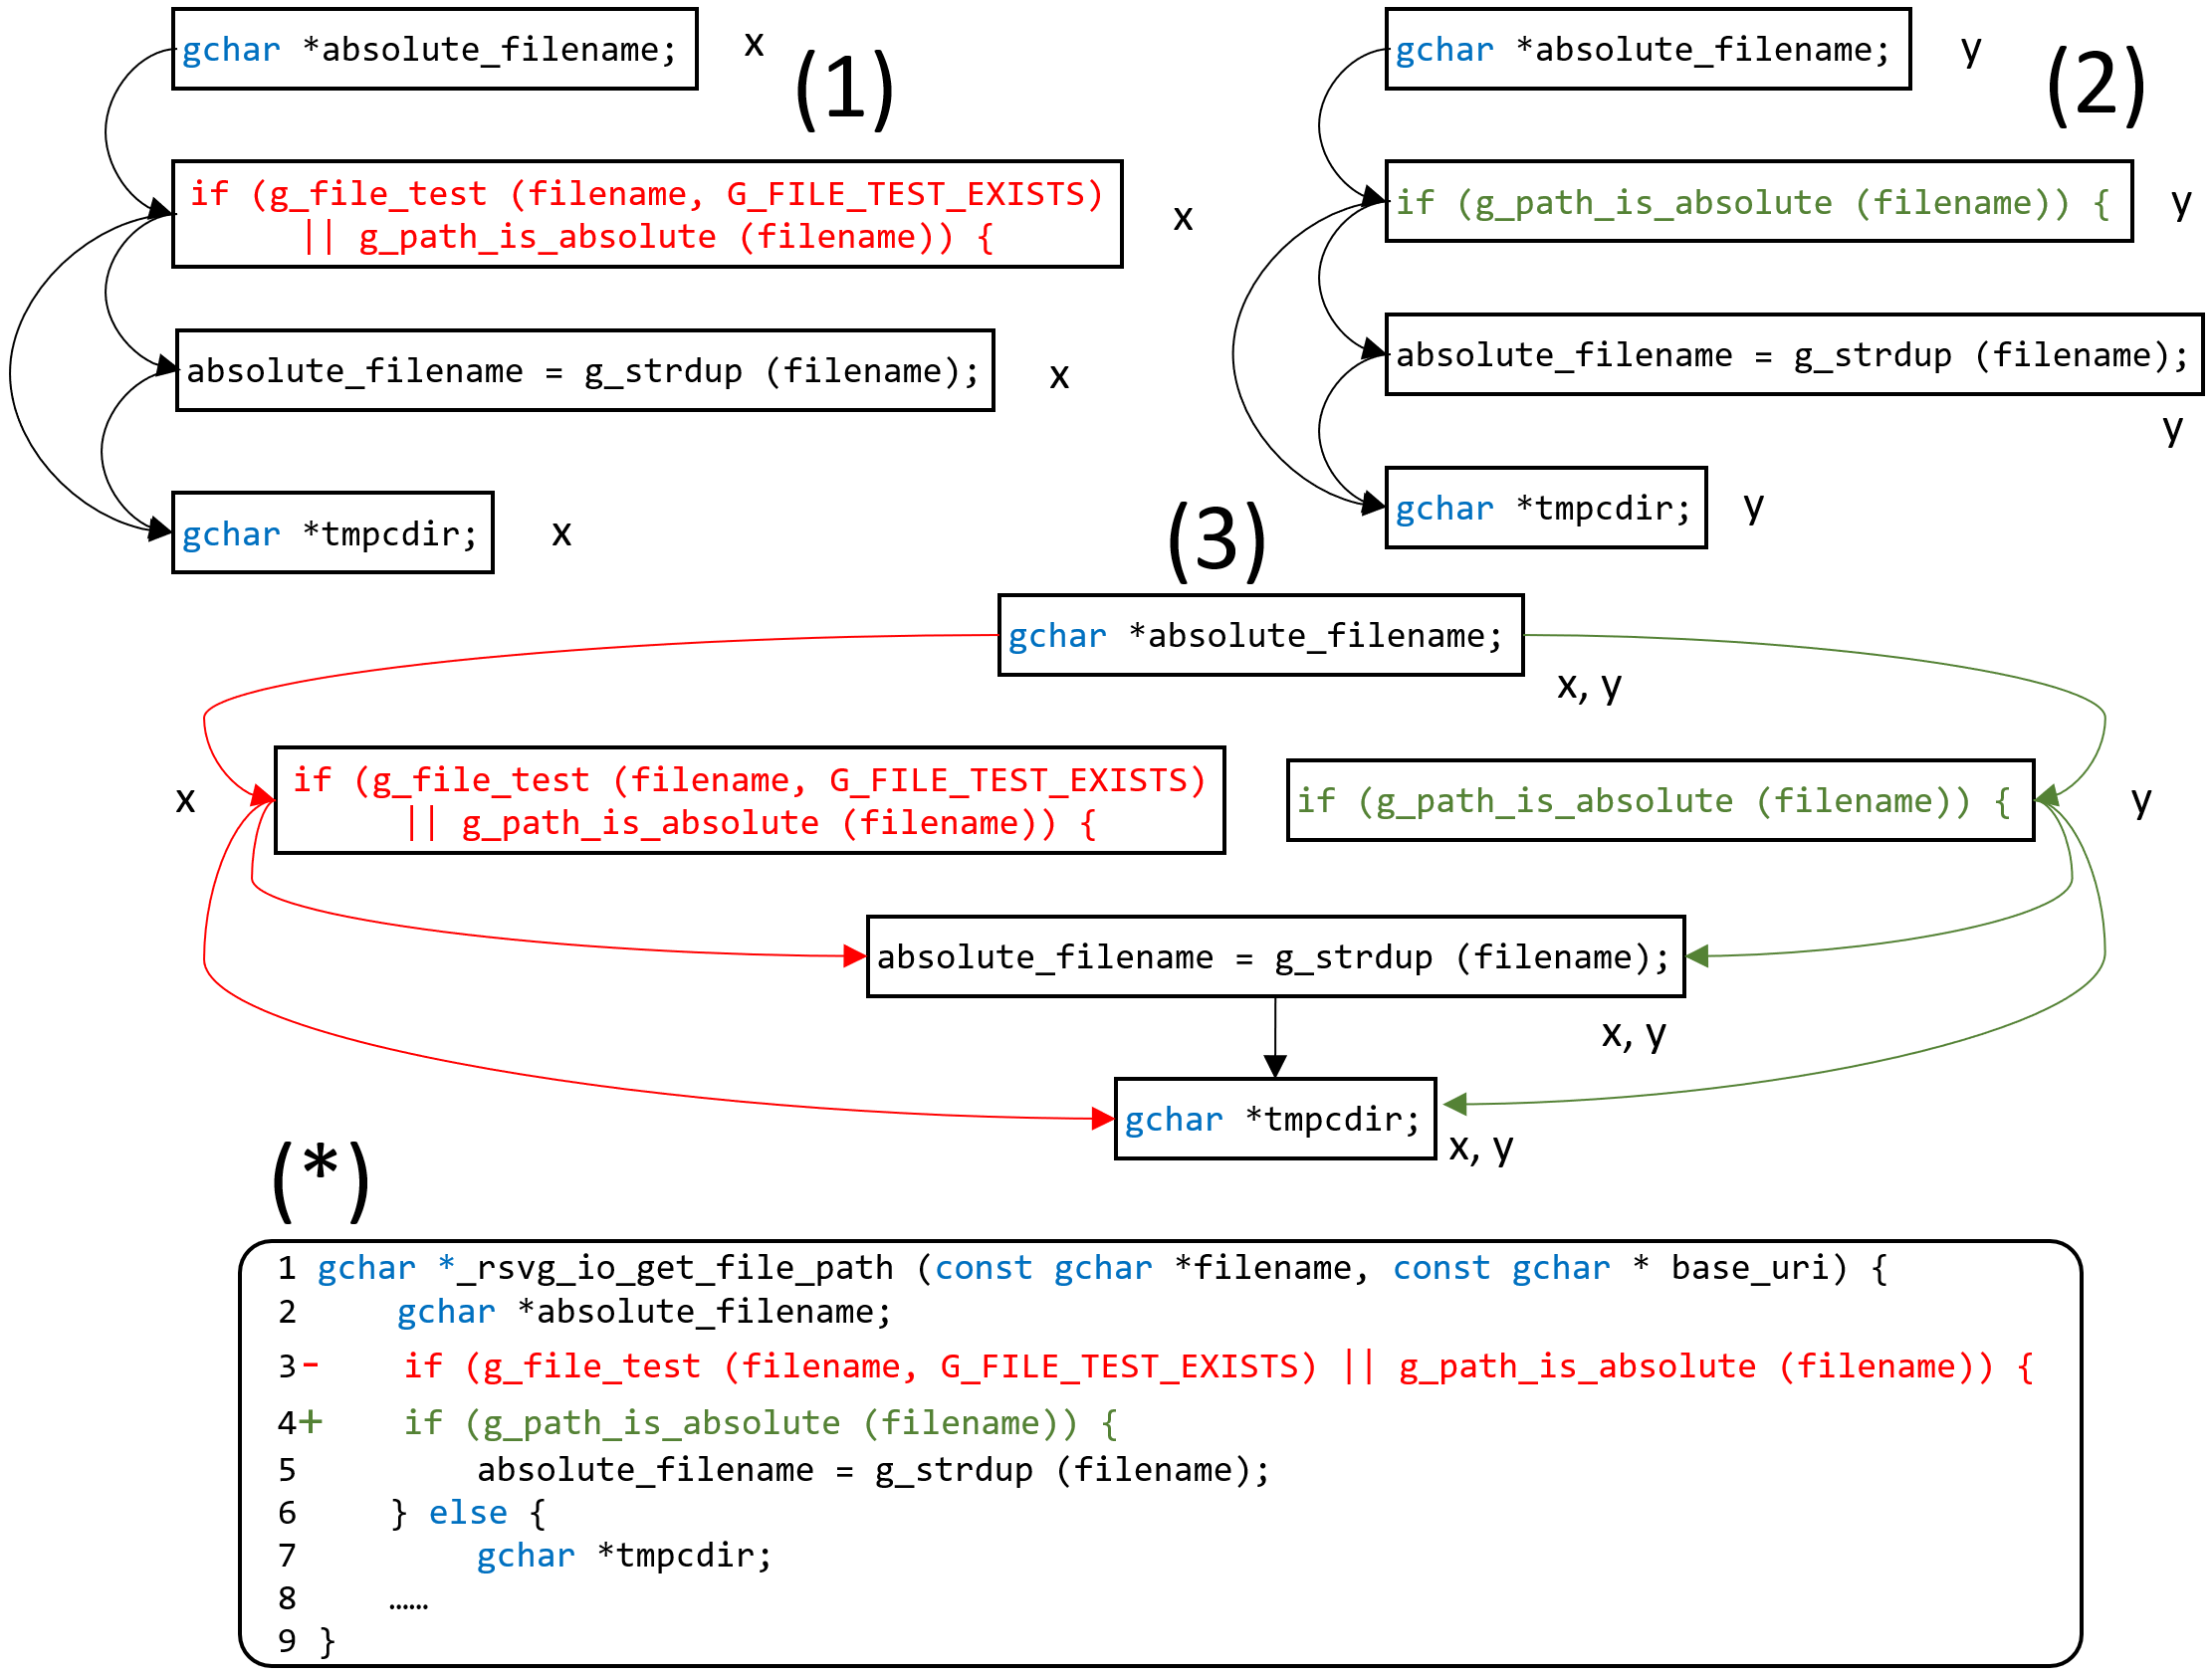
\includegraphics[width=3.4in]{graphs/multi-version-pdg.png}
	\vspace{-16pt}
	\caption{Multi-Version Program Dependence Graph}
%        \vspace{-12pt}
	\label{fig:multi-version-pdg}
\end{figure}

%Let us next explain {\tool} in details.
The first step in {\tool} is to build the multi-version PDG.
%({\mvpdgxy}).
Figure~\ref{fig:multi-version-pdg}(*) shows the vulnerable method
\code{rsvg\_io\_get\_file\_path}. The change at line 3 into line 4 was
deemed as a vulnerability-introducing change by a detection tool, in
which \code{g\_file\_test(filename,} \code{G\_FILE\_TEST\_EXISTS)} was
removed from the condition at line
3. Figure~\ref{fig:multi-version-pdg}(1)
and Figure~\ref{fig:multi-version-pdg}(2) display the PDGs of the method
\code{rsvg\_io\_get\_file\_path} before and after the change. All the
nodes of the PDG before the change are marked with $x$, and those of
the PDG after the change are marked with
$y$. Figure~\ref{fig:multi-version-pdg}(3) shows the multi-version
PDG ({\mvpdgxy}) built from the two versions $x$ and
$y$ of that method before and after the change. In {\mvpdgxy}, the
nodes labeled with either $x$ or $y$ appear only in the PDG of the
version $x$ or $y$, respectively. The nodes labeled with ($x,y$)
appear in the PDGs at both versions.



%The first step of \tool is to use before and after versions of
%vulnerability bring in commits to build the {\mvpdgxy} graph. The
%{\mvpdgxy}\cite{flexeme-fse20} is a directed graph generated from the
%disjoint union of all nodes and edges in the version $x$ and the
%version $y$ of the programming dependency graph (PDG). For example,
%Figure~\ref{fig:multi-version-pdg} shows the code change in a
%vulnerability bringing commit in which part of the if condition
%\code{g\_file\_test(filename, G\_FILE\_TEST\_EXISTS)||} is
%removed. The top left and right figures in
%Figure~\ref{fig:multi-version-pdg} display the PDG of the method
%\code{rsvg\_io\_get\_file\_path} before (we call it version $x$) and
%after (we call it version $y$) the commit changes. The statements in
%the top left figure are marked as $x$ while the statements in the top
%right figure are marked as $y$. The big figure in the middle of the
%Figure~\ref{fig:multi-version-pdg} shows the {\mvpdgxy} in which the
%deleted/added statements are marked as $x$ or $y$ and the unchanged
%statements marked as $x, y$.

We adopt the multi-version graph building algorithm in
Flexeme~\cite{flexeme-fse20}. Specifically, we generate the PDGs
for both versions~$x$ and $y$. We run Git diff tool on the source
code to determine~the changed and unchanged nodes for the
statements. The added nodes are kept in $\delta$-PDG$^{x,y}$ with the
labels $y$ as they appear in the newer version $y$. We also retain the
deleted nodes and use the label $x$ for them. The unchanged nodes
between the versions are matched by using string similarity among the
respective statements to filter the candidates and line-span proximity
to rank them. When considering the edge changes, we back-propagate the
delete nodes to the edges flowing into them. We also add all unmatched
edges in the newer version $y$ to the PDG$^{x,y}$ as the edges
relevant to the added nodes.

%Details on building $\delta$-PDG$^{x,y}$ can be found in~\cite{flexeme-fse20}.



After building $\delta$-PDG$^{x,y}$, for each changed node in the
graph, \tool collects all the unchanged nodes within the $k$-hops and
the inducing edges among them to build a sub-graph as the context for
the changed node. $\delta$-PDG$^{x,y}$ and the context for each
changed node are used as the input of the Label-GCN. Building
$\delta$-PDG$^{x,y}$ and contexts is needed in both training and
predicting.

%To build the {\mvpdgxy}, we follow the procedure from Flexeme~\cite{flexeme-fse20}. Specifically, we first generate the PDGs for both versions $x$ and $y$ of the source code. Secondly, we use the code diff tool to determine the changed (Including addition and deletion. The modified statement is regarded as one addition plus one deletion.) and unchanged statements between version $x$ and $y$. Thirdly, as for the changed statements, if the statements are added, \tool mark them as $y$ because they appear in the later version $y$, and if the statements are deleted, \tool marks them as $x$. As for the unchanged statements, \tool matches them by using string similarity among the respective statements to filter the candidates and line-span proximity to rank them. Fourthly, to consider the edges between two versions, \tool back-propagates the delete nodes (statements) to the edges flowing into them. We also add all unmatched edges in the newer version $y$ to the {\mvpdgxy} as the edges relevant to the added nodes (statements). More details on building {\mvpdgxy} can be found in~\cite{flexeme-fse20}.
